\documentclass[12pt]{article}
\rmfamily
\usepackage[margin=1.0in]{geometry}
\usepackage{graphicx}
\graphicspath{ {figures/} }

\title{TCP Dynamics Report}
\date{November 2020}
\author{Will Goodman}

\begin{document}
\maketitle

\section{Analysing the strategy of the client and server to maintain throughput on ports 4030 through 4039}
\subsection*{Investigation}
The data for this part was collected during the between 8PM and 11PM on the evening of Sunday 1st November.

\subsubsection*{Low loss, small file (Port 4032, 256KB)}
To begin investigating the strategy of the client and server, I analysed how a 256KB file was downloaded from port 4032 (10\% packet loss).
Initial inspection revealed the following:
\begin{itemize}
  \item The client's buffer is 64240 bytes
  \item Each TCP packet payload received from the server is 1452 bytes
  \item The sequence number of the packet is the cumulative number of payload bytes, including the current packet
  \item The cumulative acknowledgements from the client to the server refer to the next expected packet, not the most up-to-date received packet
  \item The client sends an ACK after every two packets have been received
\end{itemize}

By reviewing a graph of the throughput, we can see "plateaus" where no data is being transfered (figure \ref{figure1: 4032:256KB Throughput}).

\begin{figure}[!htbp]
  \centering
  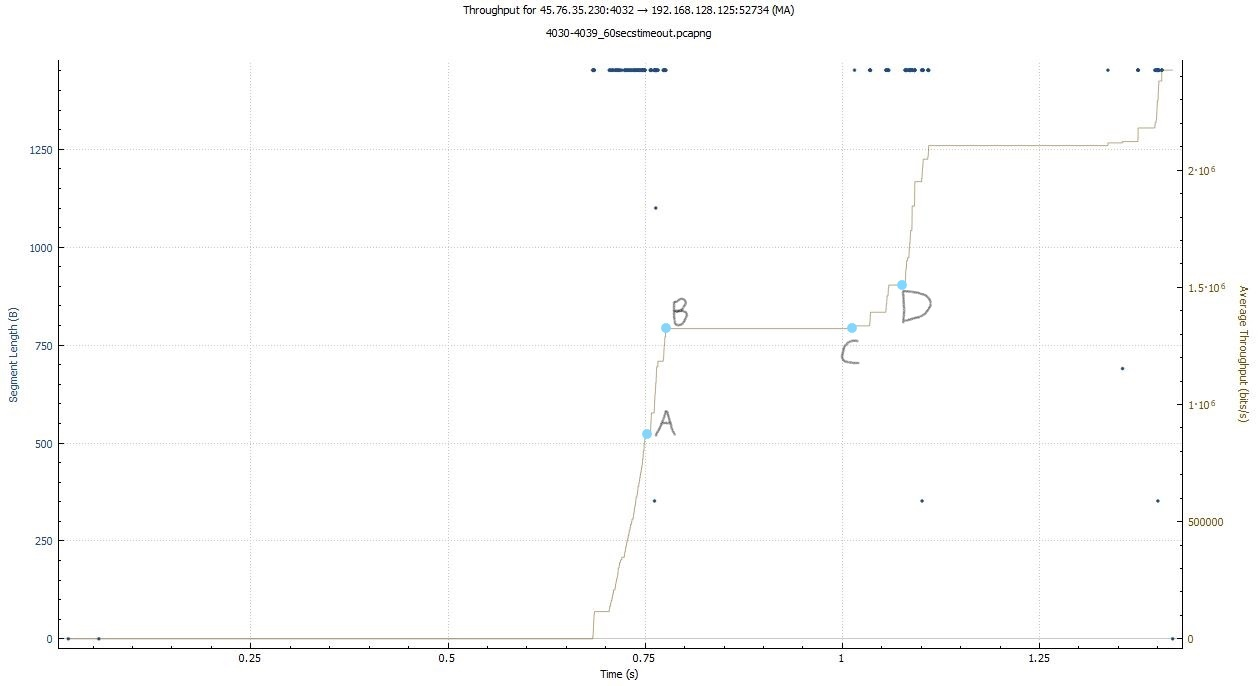
\includegraphics[scale=0.3]{4032_256KB_throughput-marked-points.jpg}
  \caption{"256KB file, port 4032 (10\%) packet loss throughput."}
  \label{figure1: 4032:256KB Throughput}
\end{figure}

Upon reviewing the packet capture, we can see that the throughput has a slight reduction when the first duplicate ACK is sent (packet 21734 in figure \ref{figure2: first duplicate ACK} is point A in figure \ref{figure1: 4032:256KB Throughput}).
Following the first duplicate ACK, it appears the server continues to send packets for 25 milliseconds before resending the missing packet.
The server keeps sending new packets, despite the client returning duplicate ACKs stating a packet has not arrived.
The server must be pipelining packets.

\begin{figure}[!htbp]
  \centering
  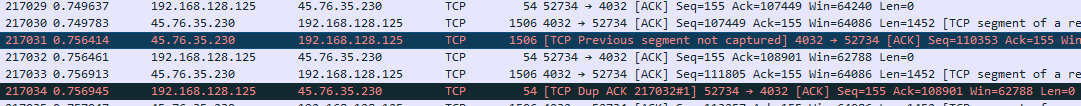
\includegraphics[width=\linewidth]{4032-256KB-duplicate-ack.PNG}
  \caption{"First duplicate ACK."}
  \label{figure2: first duplicate ACK}
\end{figure}

By looking at figure \ref{figure3: BIF and Window Size}, we can see that the number of bytes-in-flight never exceeds the Window Size, and as such the buffer in the client does not overflow.
The peak of the BIF (where the buffer would overflow), is the point where the server retransmits the missing packet.
From this we can assume that the server limits the number of unacknowledged packets which have been sent to not exceed the client's buffer space.
This is TCP flow control in action.

\begin{figure}[!htbp]
  \centering
  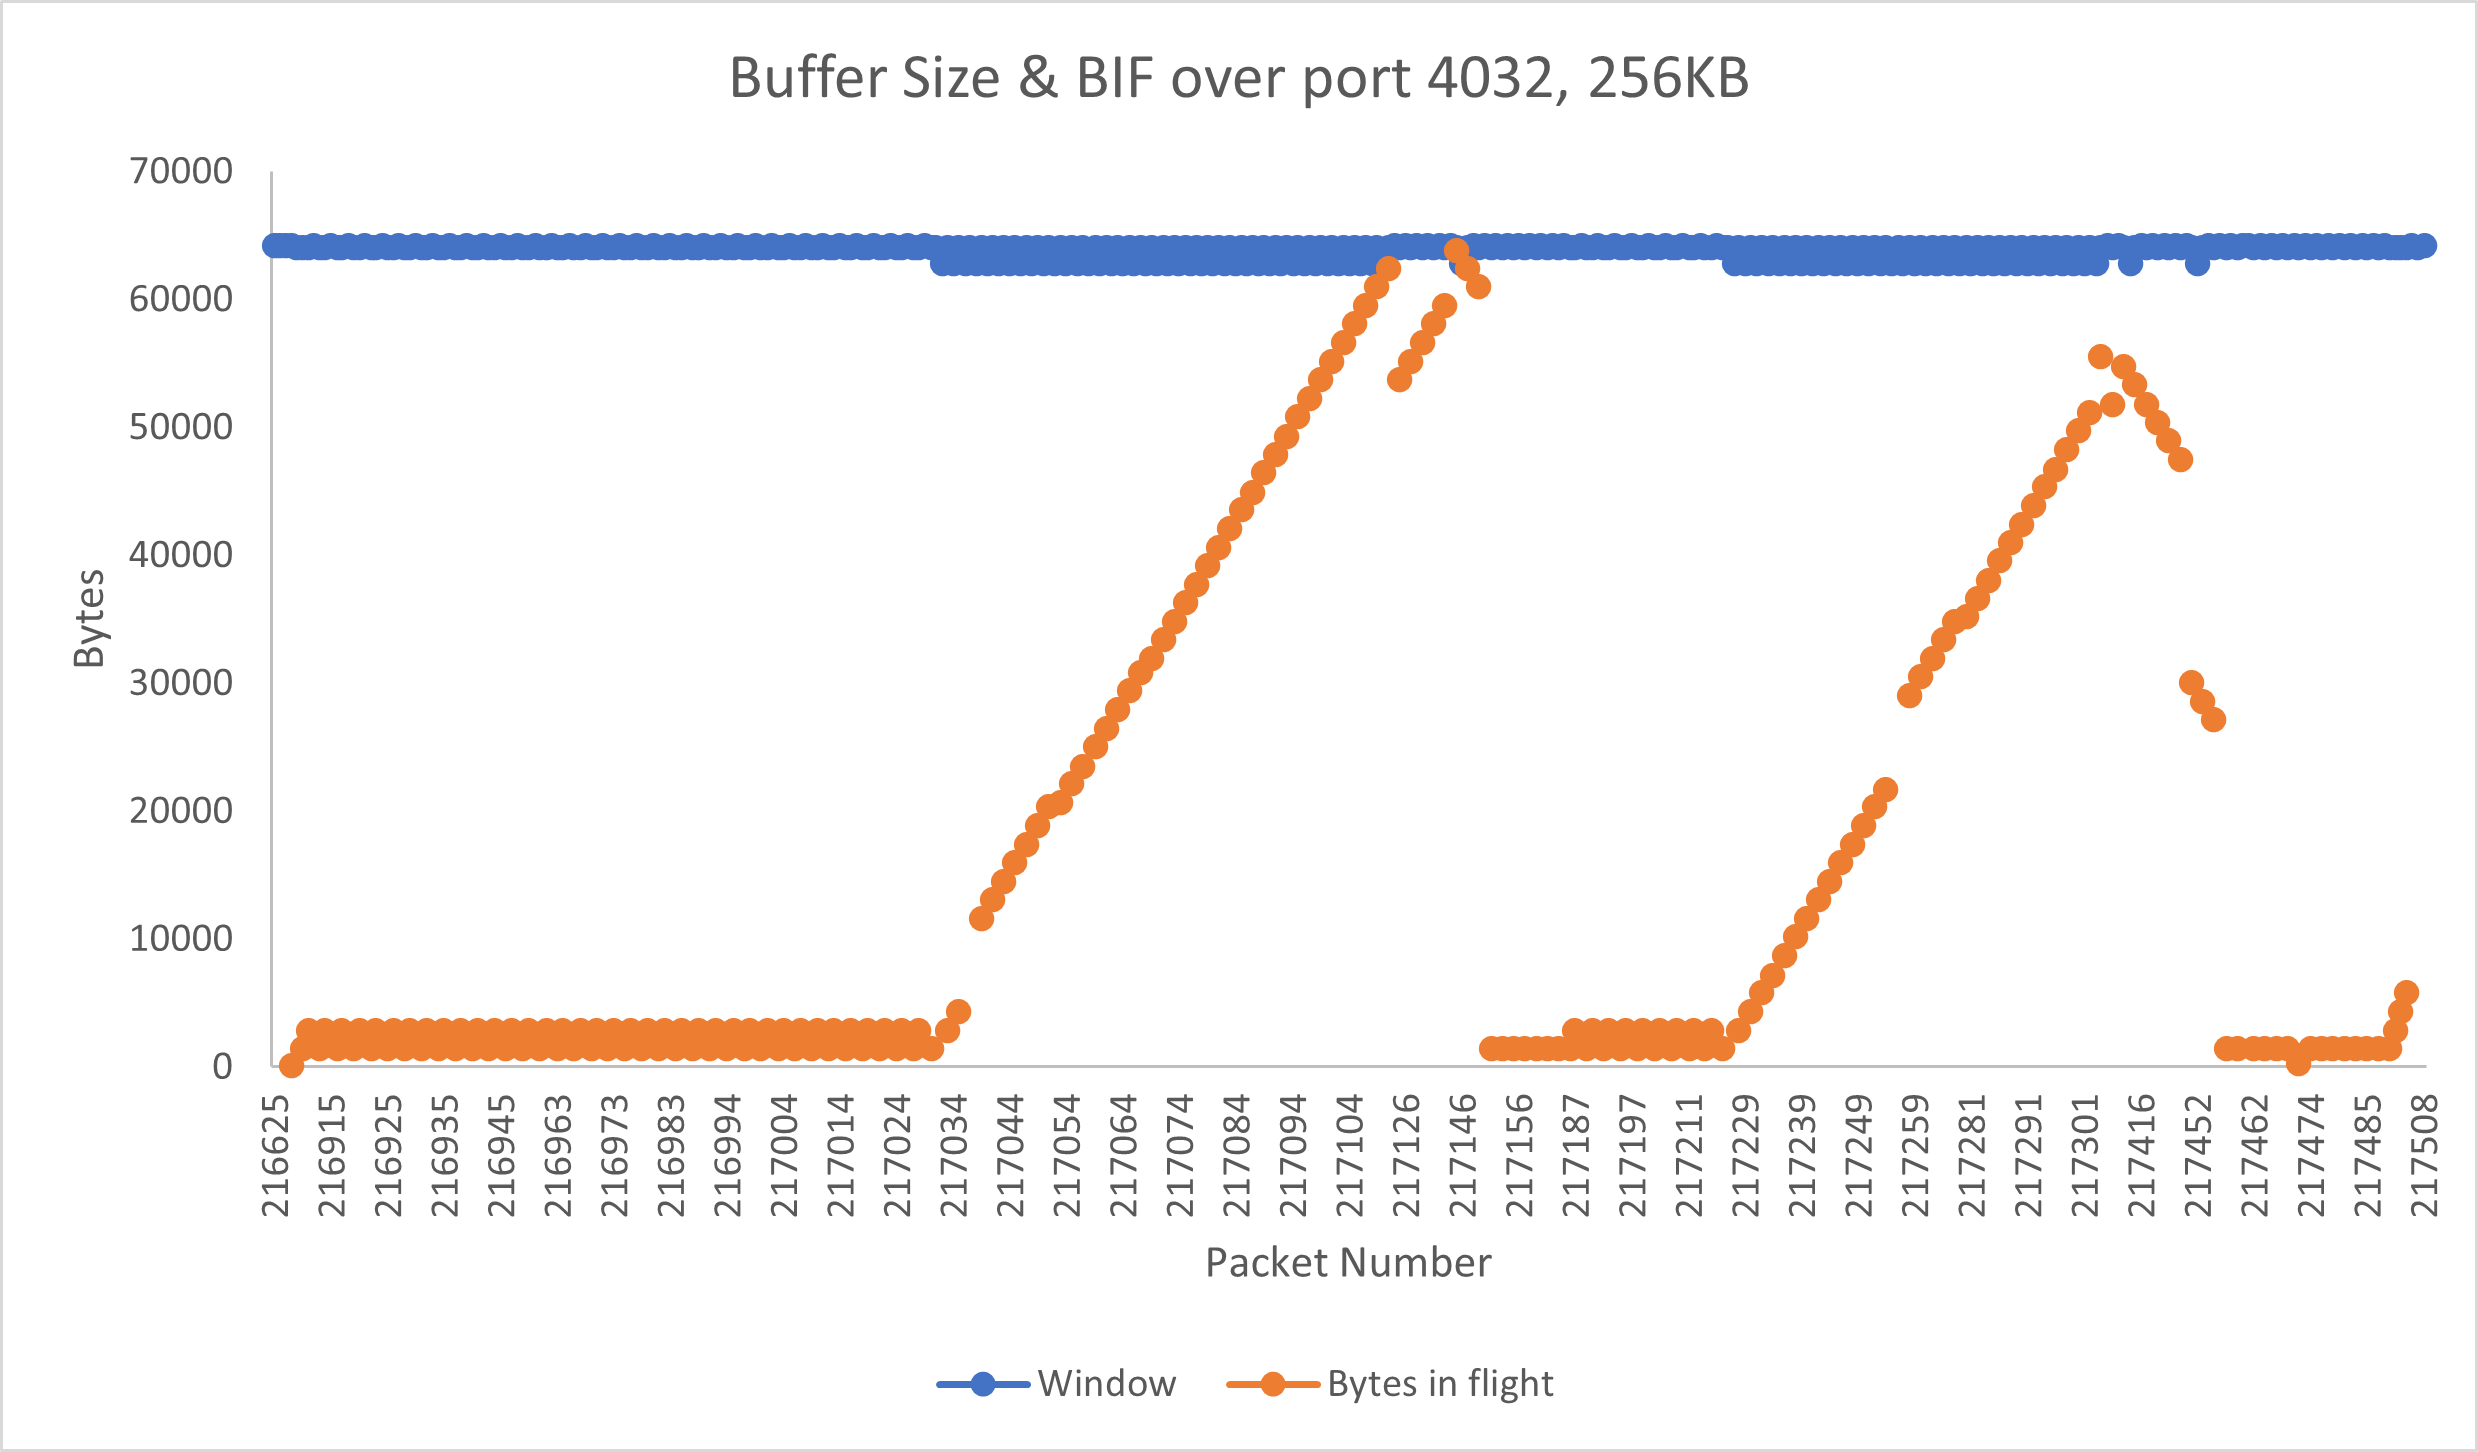
\includegraphics[width=\linewidth]{4032-256KB-bytes-in-flight.png}
  \caption{"Bytes-in-Flight in comparison to Window Size."}
  \label{figure3: BIF and Window Size}
\end{figure}

As the server simply retransmits the missing packet, rather than performing a fast retransmission, we can assume that the retransmission was caused by the acknowledgement timeout.
By looking at the time taken between the client sending the oldest ACK for the first time, and when the retransmission is received, we can estimate the timeout for unacked packets on the server.
In figure \ref{figure2: first duplicate ACK} line 217032 (ACK) is at 0.756461 seconds and in figure \ref{figure4: First retransmission} line 217113 (retransmission) is at 1.015436 seconds.
This is a time difference of 0.258975.
Later in the TCP trace another packet goes missing, and the time difference is 0.250174.
From these two values we can estimate that the timeout for the oldest unacked packet on the server is a quarter of a second, at which point the server retransmits that packet.

Once it has resent the missing packet, the server continues where it left off and continues sending packets it has not already sent.
This is seen in figure \ref{figure4: First retransmission}, where the server transmits 169885, then retransmits 108901.
Retransmission of 108901 is point C in figure \ref{figure1: 4032:256KB Throughput}
This first packet the server sends after the retransmission is 171337, which is the next in the sequence (169885 + 1452 = 171337).
This shows that the server knows the client is buffering all out-of-order packets, and is not discarding them like a pipelined receiver.

\begin{figure}[!htbp]
  \centering
  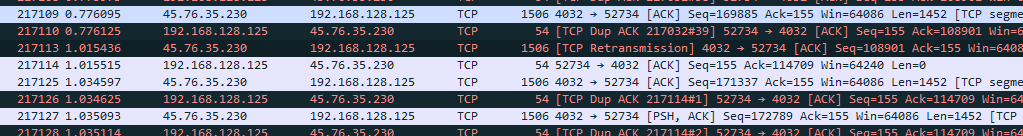
\includegraphics[width=\linewidth]{4032-256KB-retransmission.PNG}
  \caption{"First retransmission."}
  \label{figure4: First retransmission}
\end{figure}

In this case something interesting happens.
It appears a second packet had actually gone missing (114709), and so the client sends another duplicate ACK.
As the client receives more out-of-order packets, four more duplicate ACKs are sent.
On the server, this appears to trigger a Rapid Recovery/Fast Retransmission as the server starts retransmitting every packet after 114709 (see figure \ref{figure4: Fast retransmission}).

\begin{figure}[!htbp]
  \centering
  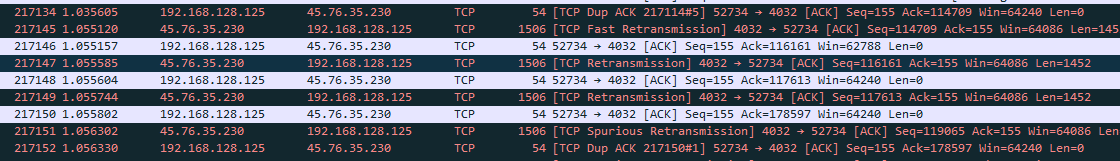
\includegraphics[width=\linewidth]{4032-256KB-fast-retransmission.PNG}
  \caption{"Fast retransmission."}
  \label{figure4: Fast retransmission}
\end{figure}

As a cumulative acknowledgement is being used, the server only knows that every packet up to 114709 has been received, it does not know the status of every packet it has sent since.
As three duplicate ACKs have been received for the same missing packet, a Fast Retransmission is triggered and every packet since the missing packet is retransmitted.
In this case, only four packets went missing (108901, 114709, 116161, 117613), and so every packet after this has already been received and buffered (causing a spurious retransmission).
Eventually, the server receives one of the client's duplicate ACKs stating that all of these packets have already been received, and the server starts sending packets as normal (figure \ref{figure5: Return to normal}, and point D on \ref{figure1: 4032:256KB Throughput}).

\begin{figure}[!htbp]
  \centering
  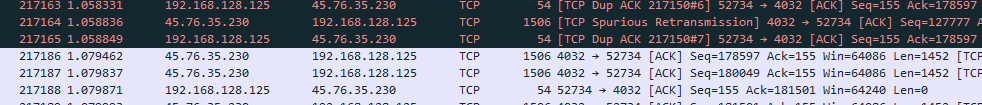
\includegraphics[width=\linewidth]{4032-256KB-back-to-normal.PNG}
  \caption{"Return to normal."}
  \label{figure5: Return to normal}
\end{figure}

The question arises, why did the first missing packet not cause a Fast Retransmission but the second did?
This may be because some or all of the duplicate acknowledgements for the first missing packet never arrived at the server, or did not arrive before the timeout.
The same reason may be why five duplicate acknowledgements were sent before the Fast Retransmission of the second missing packet was triggered, as opposed to the three duplicate ACKs required by the specification. 

Further evidence of this appears lower within the same TCP stream (figure \ref{figure6: Missing ACKs}), a collection of packets are retransmitted despite acknowledgements being sent by the client.
The packets must be timing out as the ACKs are not arriving at the server, causing them to be retransmitted even though they have already been acknowledged by the client (spurious retransmission).
The duplicate ACKs for packet 232321 must arrive however, as the Fast Retransmission is triggered for that packet.

\begin{figure}[!htbp]
  \centering
  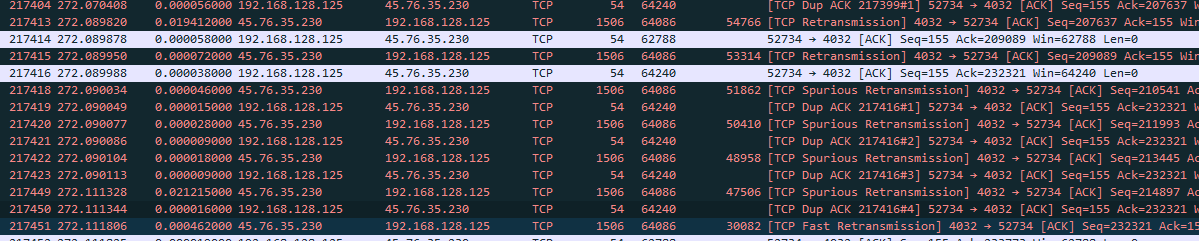
\includegraphics[width=\linewidth]{4032-256KB-lost-acks.PNG}
  \caption{"ACKs going missing."}
  \label{figure6: Missing ACKs}
\end{figure}

Another feature which is worth noting, is the server does not appear to be using Slow Start.
This is unexpected, as Slow Start is compulsory.
In figure \ref{figure3: BIF and Window Size} we can see that the number of bytes-in-flight stays stable at 2904, unless a packet has been unacknowledged.
If Slow Start was in use, we would expect to see this increase exponentially until a packet has been lost.

\subsubsection*{Low loss, medium file (Port 4032, 16MB)}
With a larger file, we begin to see how both the client and server deal with packet loss over a longer period of time.
% By reviewing the Stevens Time Sequence, we can clearly see that Slow Start is being used. 
% This is not surprising as it is compulsory under the TCP specification.

% \begin{figure}[!htbp]
%   \centering
%   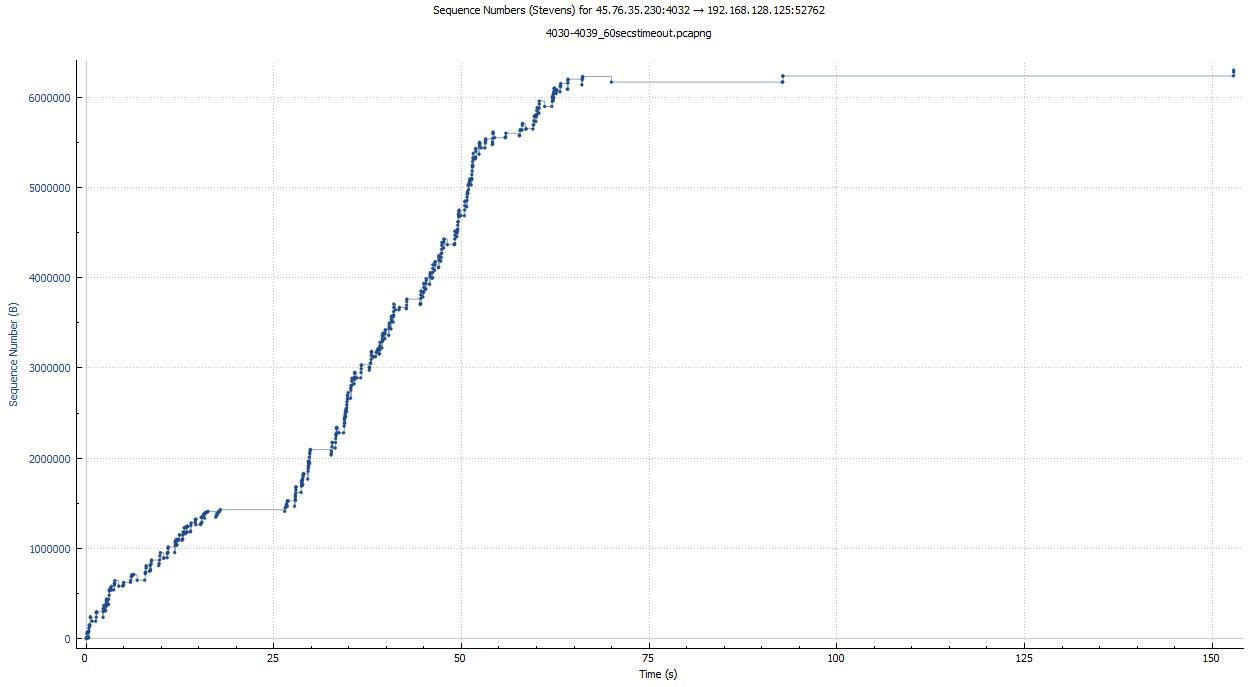
\includegraphics[width=\linewidth]{4032-16M-stevens.jpeg}
%   \caption{"16MB file, port 4032 (10\%) packet loss stevens."}
%   \label{figure6: 4032:16M Stevens}
% \end{figure}

By looking at the packet capture, we can see that the same behaviour of acknowledgements and retransmissions occurs for the larger file as it did for the smaller file.
The Window size advertised by the client is large (64240 Bytes) and the buffer never fills up, and as such we never see if Silly Window Syndrome occurs.
This does show however, that Silly Window Syndrome is not as much of an issue today with faster processing power and larger memory.

This 16Mb file never actually finished downloading, the client ended the connection before it completed (figure \ref{figure7: 4032:16M RST}).

\begin{figure}[!htbp]
  \centering
  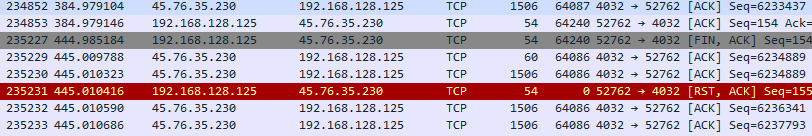
\includegraphics[width=\linewidth]{4032-16M-RST.PNG}
  \caption{"Client RST."}
  \label{figure7: 4032:16M RST}
\end{figure}

Upon further inspection we can see the last contact from the server (234852) is at 384.979104 seconds.
60 seconds later (235227), the client sends a FIN, ACK packet to close the connection.
This is triggered by the timeout within the Python script used to collect the data (shown at the start of the report).
After this FIN, ACK packet, the client receives a regular packet from the server. 
This packet was likely already in the wire when the FIN, ACK was received by the server.
Due to this, the client sends a RST, ACK packet to terminate the connection completely.

\subsection*{Client/Server Strategy}
\subsubsection*{Client}
Following the investigation, I believe this is the Client's strategy to attempt to maintain throughput:
\begin{itemize}
  \item Send a cumulative ACK after receiving every two packets
  \item If an out-of-order packet is received, an ACK is sent stating what the next expected packet is
  \item If another out-of-order packet is received, a duplicate ACK is sent. This repeats until the missing packet is received
  \item All out-of-order packets are buffered
  \item If a duplicate packet is received, then a duplicate ACK is sent
  \item When the last packet arrives, send a FIN, ACK to close the connection
  \item If no packets from the server for 60 seconds, send a FIN, ACK to close the connection
  \item If any packets are received from the server after sending a FIN, ACK (excluding an acknowledgement of the FIN, ACK), send a RST, ACK packet
\end{itemize}

\subsubsection*{Server}
The server knows less about which packets have been received correctly than the client, so it has a slightly more complicated strategy.
\begin{itemize}
  \item Send packets in order, pipelining packets without waiting for acknowledgement
  \item Use a congestion window of 2 packets
  \item If a packet has not been acknowledged after quarter of a second, just resend that packet. Assume all packets sent since that packet have arrived correctly and pick up where you left off after it is resent
  \item If you receive three duplicate ACKs for a packet, assume all packets from that sequence number on have been lost and resend them all (Rapid Recovery)
  \item If you receive a duplicate ACK from the client stating that more packets have been arrived than previously thought, stop resending packets before that sequence number and start sending subsequent packets
  \item If you receive a FIN, ACK from the client, as all packets have been received correctly (or the client wants to stop the connection for another reason)
\end{itemize}

\section{Analysing Drop In Performance As Packets Are Lost}

\end{document}